
    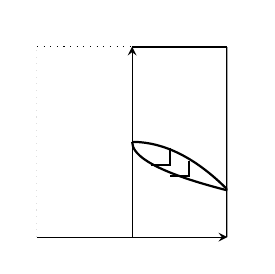
\begin{tikzpicture}
        \begin{axis}[
            axis lines = middle,
            xlabel = $ $,
            ylabel = $ $,
            xmin = -0.5, xmax = 0.5,
            ymin = 0, ymax = 1,
            xtick = {0},
            ytick = {0},
            x label style={at={(axis description cs:1,0)},anchor=west},
            y label style={at={(axis description cs:0,1)},anchor=south},
            extra tick style={grid=major},
            width=4cm, height=4cm,
            samples=100,
            domain=-0.5:0.5,
        ]
\draw [thick](0.5,0) -- (0.5,1);
\draw [thick](0.5,1) -- (0,1);
                \addplot[domain=0.1:0.2, samples=100, thick] {0.38};
                \addplot[domain=0.2:0.3, samples=100, thick] {0.32};
           \draw [dotted](-0.5,0) -- (-0.5,1);
\draw [dotted](-0.5,1) -- (0,1);
\draw [dotted](0,0) -- (-0.5,0);
        \draw [thick](0.2,0.47) -- (0.2,0.38);
                          \draw [thick](0.3,0.40) -- (0.3,0.32);





        \addplot[domain=0:0.5, samples=100, thick] {0.5-x^2};
                \addplot[domain=0:0.5, samples=100, thick] {(-(0.36*x^(0.5))+0.5};




        \end{axis}
    \end{tikzpicture}
    
